\chapter{Background}
 High-performance computing is the use of multiple processors or computers for running compute advanced applications efficiently, reliably and quickly with high throughput. Over the past few years high-performance computing has evolved considerably because of the emergence of CPU-GPU heterogeneous architectures. In this work, High performance computing techniques are used to implement the computer vision, image processing and autonomous drive algorithms.
% section 1.1
\section{Need for high-performance computing}
Modern CPU's are designed such that power available was plentiful and complete performance was the important figure of merit. The resulting architectures are highly optimized for single-thread performance with the features such as out-of-order execution, branch prediction, and large primary instruction and data caches. In such type of designs, most of the power is used for data movement overheads, supplying the instructions and control mechanisms [5].\paragraph*{} The accessing time for on-chip static RAM(cache) is less than(~200 times) the time accessing time for DRAM. Current programming practices mainly focus on sequential, homogeneous machines with a flat view of memory. With explicit control over the data movement within the memory hierarchies will result in performance sensitive code practices. Conventional architectures has a flat view of memory by having implicit data caching at multiple levels, such a practice is not sustainable for scalable systems \cite{ProfessionalCUDA}.
\paragraph*{} The data accessing latencies in the machine will be hidden by adapting to parallel processing, especially data and fine-grained thread parallelism. In this work, these parallel processing techniques are implemented for algorithms to gain good performance. A sequence of instructions is called a thread. Conventional programming systems don't provide a convenient means of providing tens of, tens of thousands of threads (or even more) on a single die. A system with such attributes is needed for parallel processsing. A system with different kinds of processors which are complement to each other in performance comprises a heterogeneous system. In a heterogeneous system, individual processors will have processing elements with different performance characteristics, different views of the memory, and will have different levels of physical parallelism \cite{ProfessionalCUDA}. 
\paragraph*{} The high performance computing techniques can be used for multi-core CPUs and many-core GPUs. In this work both are discussed. Hetereogeneous parallel computing is used for CPU-GPU platform, whereas multi-core computing is used for CPU only platform. The algorithms adaptive contrast enhancement, motion de-blur and stereo disparity block matching are implemented using heterogeneous parallel computing. Fog rectification and temporal denoising are implemented using multi-core programming. 
\section{Heterogeneous parallel computing}
Heterogeneous parallel computing is a hybrid word derived from two paradigms, heterogeneous computing and parallel computing. It is the processing of data in parallel using heterogeneous architecture.
\subsection{Parallel computing}
 Parallel computing is a form of computing, in which many computations are performed simultaneously. It is motivated by the fact that a large problem can be broken down into smaller ones, and all of them are solved concurrently. From the programmer’s point of view, it is mapping those parallel computations to the available compute resources \cite{ProfessionalCUDA}.
\subsection{Types of parallelism}
 The parallel execution of an algorithm gives good utilization of hardware resources and the application performs in real time. There exist mainly two types of parallelism in an application, task level parallelism and data level parallelism. The algorithm which is to be implemented using parallel computing should be analysed properly for the type of parallelism it supports.
\begin{description}
\item[Task-level parallelism] \hfill \break It is applicable if there exist many independent tasks or functions in an algorithm. For example, if there are three tasks in an application such as decoding video, processing video, and displaying the output. Even though each task has dependency with each other, they can be made independent by executing them using a three stage pipeline on different cores. We have used this methodology in implementing computer vision algorithms on a Rcar-H3 SoC which has an active quad-core ARM A-57.
\item [Data parallelism] \hfill \break  On the other hand, Data parallelism is possible when there exist many data elements that can be operated independently \cite{alantatourian}. It focuses mainly on distributing data elements to multiple threads on multiple cores. This Data level parallelism is most useful in heterogeneous programming where the hardware contains a complementary coprocessor which is capable of handling the execution of multiple data elements at once. We followed CUDA programming to address the data parallel portions in the algorithms. The computer vision and image processing algorithms implemented in this work are used data parallelism.
\end{description}
\subsection{Heterogeneous computing}
Heterogeneous computing refers to systems that use multiple types of processors. Heterogeneous System Architecture (HSA) systems use multiple types of processors (typically CPUs and GPUs), usually on the same silicon chip or added discretely to the central processor \cite{amd}. GPU processing, aside from the well-known 3D graphics rendering, can be used for Mathematically intensive calculations on vast amounts of data, while CPUs can run the operating system and perform traditional serial tasks. GPU is added to a system as a coprocessor to CPU, which supplements its functionalities for the tasks where CPU overloads. This brings a new world of computing where the compute and bandwidth intensive tasks offload the CPU, and the CPU continues it's sequential execution smoothly. This type of architecture is used in this work, where CPU is Intel i5@3.0GHZ and GPU is NVIDIA GeForce GT640 with 384 cores.
\subsection{Heterogeneous architecture}
Currently, GPU is not a standalone platform, but it is attached to CPU as a coprocessor through a PCI-Express bus so that it will work in conjunction with CPU. The CPU monitors all the GPU activities. CPU is called a host and GPU a device. The Figure \ref{Figure:1.1} shows the CPU-GPU environment.
\begin{figure}[h!]
  \centering
  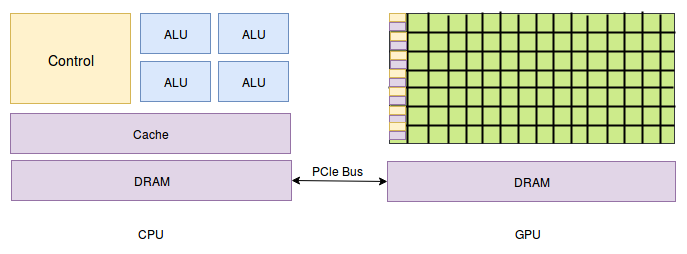
\includegraphics[width=0.8\linewidth]{HeteroGeneousArch.png}
  \caption{Heterogeneous architecture \cite{ProfessionalCUDA}}
  \label{Figure:1.1}
\end{figure}
In a heterogeneous application, there are two types of portions, a host code that runs on CPU and a device code that runs on GPU. Allocating suitable portions of code for CPU and GPU makes the application perform in real time. CPU initializes the heterogeneous application and will manage environment, data and code to the device. The sequential parts of the application execute on the CPU and the intensive data parallel parts run on the GPU as shown in the Figure \ref{Figure 1.2}. 
\begin{figure}[h!]
  \centering
  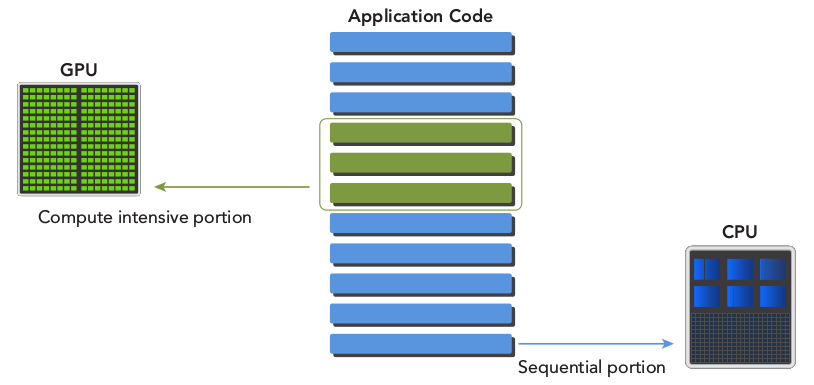
\includegraphics[width=0.75\linewidth]{seq-parallel.png}
  \caption{Distributing the Heterogeneous code to the suitable processor\cite{ProfessionalCUDA}}
  \label{Figure 1.2}
\end{figure}
\paragraph*{} In the heterogeneous architecture, the GPU may be integrated into the processor or added externally to the CPU. For this work a desktop PC with NVIDIA GPU is used. NVIDIA GPU is preferred for this work because of its ease of programming. A term is coined for using GPU for general purpose programming, which is GPGPU(General purpose programming on Graphics Processing Unit). GPGPU is supported through frameworks such as OpenCL,CUDA etc. Compute Unified Device Architecture (CUDA) is predominant now a days because of its simple and efficient APIs, it is used to program NVIDIA GPUs. The following product families of NVIDIA exhibit the GPU computing platform.
\begin{enumerate} 
\item \textbf{GeForce} \hfill \break It is designed especially for consumer graphics.
\item \textbf{Quadro} \hfill \break This product family is suitable for professional visualization.
\item \textbf{Tesla} \hfill \break This family of products mainly used for parallel computing at data center .
\item \textbf{Tegra} \hfill \break It is designed specially for mobile and embedded computing platforms.
\end{enumerate}
NVIDIA GPUs are classified within the product family according to their architectures such as Fermi,Kepler, Maxwell and Pascal. Each architecture has their own benefits from the previous architectures. In this work Kepler architecture NVIDIA GPU is used. The selection of suitable GPU platform is based upon the following important features.

\begin{itemize}
\item Number of GPU cores
\item Memory size
\end{itemize}

\section{NVIDIA GPU architecture}
The NVIDIA GPU contains an array of streaming multiprocessors (SM), each SM is capable of running thousands of concurrent threads, as shown in the Figure \ref{Figure:1.3}. A thread is a sequence of instructions to be executed on a processor. A group of threads are called a warp, each warp executes per each instruction cycle in an SM. Instruction level parallelism is extracted by pipe-lining the instructions in each thread. There is no branch prediction and speculative execution in GPU. NVIDIA GPUs use different types of memory for performance improvements in the Data movement. The shared memory used is local and has very less memory transaction cost. The texture and constant memories are useful for special type of applications and have efficient data movement.
\begin{figure}[htb]
	\centering
	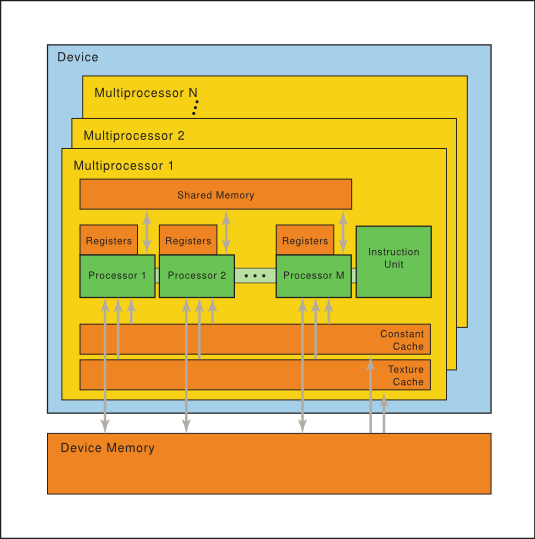
\includegraphics[width=0.8\linewidth]{hardware-model.png}
	\caption{NVIDIA GPU hardware model\cite{hwmodel}}
	\label{Figure:1.3}
\end{figure}
\paragraph*{}By Using CUDA platform one can access all the NVIDIA GPU features explained above. CUDA is becoming more significant now a days because of its simple interfaces, and is evolved as a Heterogeneous computing platform that enables the users to easily write heterogeneous programs onto NVIDIA GPU’s.